
\documentclass[11pt]{article}

\usepackage[margin=2cm,nohead]{geometry}

\usepackage{utopia}

\usepackage{color}
\usepackage[usenames,dvipsnames,svgnames,table]{xcolor}

\usepackage[authoryear]{natbib} 
\setlength{\bibsep}{0.0pt}	% remove extra line spacing bibliography entries
%\usepackage{bibentry}
%\nobibliography{references/references}

\usepackage{graphicx}

%\usepackage{hyperref}

\fontfamily{utopia}

\usepackage{textcomp}

% no paragraph indent
\setlength{\parindent}{0cm}

%\setlength{\parskip}{\baselineskip}



%\maketitle
\begin{document}
\title{\Large Groundwater flow, heat and solute transport\\
constructing your own numerical models using Python
\author{
\large Elco Luijendijk\\
\normalsize McGill University, Montreal, Canada\\
\texttt{elco.luijendijk at mcgill.ca}\\
}
\date{}
}

\maketitle


\section{Escript}

Escript is a generic finite element model that solves the following partial differential equation:

\begin{equation}
    - \nabla (A \nabla u + B u ) + C \nabla u + D u = - \nabla X + Y
\end{equation}


escript equation in Einstein notation:

\begin{equation}
    - (A_{ij} u_{j} ) _{,i} - (B_{i} u) _{,i} + C_{j} u_{,j} + D u = -(X_{,j})_{_,j} + Y 
\end{equation}

The Einstein notation for a derivative is:

\begin{equation}
    u_{,t} = {\partial u \over{\partial{t} } }
\end{equation}


\pagebreak

\subsection{Groundwater flow}


\subsection{Simplified flow equation, constant density}

For a fluid with constant density ($\rho_f$= constant), fluid flow is driven by changes in hydraulic head ($h$). Recall that hydraulic head is equal to the pressure head and the elevation head: $h = P/ (\rho_f g) + z$. If h is constant the fluid is static.

The fluid flow equation for a constant density fluid is:  

\begin{equation}
	  S_{sh}  \frac{\partial h}{\partial t} = \nabla ( K  \nabla h ) + W
\end{equation}

where $S_{s}$ is the specific storativity $m^{-1}$, which is the volume of fluid released per unit decrease in hydraulic head. $h$ is the hydraulic head [$m$], $t$ is time [$s$], $K$ is the hydraulic conductivity [$m s^{-1}$] and $W$ is a source or sink term [$s^{-1}$]. The source/sink term $W$  can be used to represent processes that add fluids to the system, such as groundwater recharge, or processes that take fluid out of the system, such as pumping.  


\subsubsection{Steady state}

Steady-state flow means that the hydraulic head is stable over time, in mathematical terms: ${\partial h \over{\partial t}} = 0$. For steady state conditions the groundwater flow equation reduces to:

\begin{equation}
	   \nabla K  \nabla h + W = 0
\end{equation}

The PDE form solved by escript/Finley is:

\begin{equation}
    - \nabla (A \nabla u {\color{gray} + B u ) + C \nabla u + D u} = {\color{gray} - \nabla X} + Y
\end{equation}

Rewriting the steady-state flow equation gives:
 
\begin{equation}
	   - \nabla \underbrace{-K}_A  \nabla \underbrace{h}_u =  \underbrace{-W}_Y
\end{equation}

And the resulting escript coefficients are: 

$ u = h $

$ A = - K $

$ Y = - W $


\subsubsection{Explicit formulation (forward in time)}

We use forward Euler discretization in time. This means that the hydraulic head at time $t = t+1$ is calculated as a function of the hydraulic head at the preceding timestep $t = t$

\begin{equation}
    {\partial h \over{\partial t}} = {h_{t+1} - h_t \over{\Delta t}} 
\end{equation}

and taking $\nabla h = \nabla h_t $ results in:

\begin{equation}
   S_{sh} {h_{t+1} - h_t \over{\Delta t}} = \nabla K  \nabla h_t + W
\end{equation}

Rearranging this in the shape of the escript equation gives:

\begin{equation}
   S_{sh} h_{t+1} =  \nabla dt K \nabla h_t + dt W + S_{sh} h_t 
\end{equation}

\begin{equation}
   {\color{gray} - \nabla (A \nabla u + B u ) + C \nabla u} + D u = - \nabla X + Y
\end{equation}

\begin{equation}
   \underbrace{S_{sh}}_D \underbrace{h_{t+1}}_u = - \nabla \underbrace{-dt K \nabla h_t}_X + \underbrace{dt W + S_{sh} h_t}_Y 
\end{equation}

The resulting coefficients of the escript PDE are:

$u = h_{t+1}$

$ D = S_{sh} $

$ X = - dt * K * \nabla h_t$

$ Y = dt W + S_{sh} h_t $

The remaining coefficients are not used:

$ A=0 , B = 0 , C = 0 $


\subsubsection{Implicit solution (backward in time)}

Here we again take $h_{t+1}$ as the unknown variable. However, this time we rewrite the equation to calculate the hydraulic head as a function of the divergence of the hydraulic head at the same timestep $\nabla h_{t+1}$. 


\begin{equation}
 	S_{sh} {h_{t+1} - h_t \over{\Delta t}} = \nabla K  \nabla h_{t+1} + W
\end{equation}

Rearranging this equations gives:

\begin{equation}
   - \nabla dt K \nabla h_{t+1} + S_{sh} h_{t+1} =  S_{sh} h_t + dt W 
\end{equation}

and again in the same notation as the escript PDE:

\begin{equation}
    - \nabla (A \nabla u + {\color{gray}B u} ) + {\color{gray}C \nabla u} + D u = {\color{gray}- \nabla X} + Y
\end{equation}

\begin{equation}
   - \nabla \underbrace{dt K}_A \nabla \underbrace{h_{t+1}}_u + \underbrace{S_{sh}}_D \underbrace{h_{t+1}}_u =  \underbrace{S_{sh} h_t + dt W }_Y 
\end{equation}



%\begin{equation}
%    f=\frac{n v}{2 L}, \underbrace{\color{red}n=1, 2, 3, \ldots}_{\text{allowed n's}}
%\end{equation}




$u = h_{t+1}$

$A = dt K$

$D = S_{sh} $

$Y = S_{sh} h_t + dt W $

\subsubsection{Setting boundary conditions}

The peceding equations solve hydraulic head in a given model domain. However, the solution always need so-called boundary conditions. The two main boundary conditions are a specified head or a specified flux at the boundary. 

A specified flux or Neumann boundary condition is in escript defined as:

\begin{equation}
	\vec n A \nabla u + {\color{gray}\vec n B u + d u} = {\color{gray} \vec n \nabla X } + y
\end{equation}

Where $u$ is again the variable we are trying to solve (hydraulic head). $\vec n$ is a vector normal (perpendicular) to the model boundary. 


The flux $q$ is given by Darcy's law: $q = K \nabla h$

If we want to define a fixed flux ($q_b$ [$m s^{-1}$]) at the boundary, the equation becomes:

\begin{equation}
	\vec n \: dt K \nabla h = q \: dt
\end{equation}

with 
$y = q \: dt $


\subsection{Density-dependent groundwater flow}

The equation for variable density groundwater flow is given by:
\begin{equation}
    \label{eq:var_density_flow}
	 S_s { \partial P \over {\partial t} } = \nabla { \rho_f k \over{\mu} } (\nabla P + \rho_f g \nabla z ) + W
\end{equation}



\subsubsection{Steady-state flow}

Governing equation for steady-state variable density flow:

\begin{equation}
	   - \nabla {\rho _{f} k \over{\mu} } (\nabla P + \rho g \nabla z) = W
\end{equation}

Separate pressure and bouyancy term:

\begin{equation}
	   - \nabla {\rho _{f} k \over{\mu} } (\nabla P )  = \nabla {\rho_{f} k \over{\mu} } \rho_f g \nabla z + W
\end{equation}

Escript PDE:

\begin{equation}
    - \nabla (A \nabla u + {\color{gray}B u} ) + {\color{gray}C \nabla u + D u } = {\color{gray}- \nabla X} + Y
\end{equation}

Reorganize steady state flow eq. and select coefficients to use in escript PDE solver:

\begin{equation}
	   - \nabla \underbrace{{\rho _{f} k \over{\mu} }}_A \nabla \underbrace{P}_u = - \nabla \underbrace{- {\rho_{f} k \over{\mu} } \rho_f g \nabla z}_X + \underbrace{W}_Y
\end{equation}

Escript coefficients:

$u = P $

$A = {\rho_f k \over{\mu} } $

$X = - {\rho_{f} k \over{\mu} } \rho_f g \nabla z$

$Y = Q $


\subsubsection{Transient flow, explicit formulation}

\begin{equation}
	 S_s { \partial P \over {\partial t} } = - \nabla { \rho_f k \over{\mu} } ( \nabla  P + \rho_f g \nabla z ) + W
\end{equation}

with discretization in time following:

\begin{equation}
    \label{eq:energy_density_explicit}
    {\partial P \over{\partial t} } \approx {P^{t+1} - P^{t} \over{dt} }
\end{equation}

gives:

\begin{equation}
	 S_s P^{t+1} = - dt \nabla { \rho_f k \over{\mu} } ( \nabla  P^{t} + \rho_f g \nabla z) + W dt + S_s P^{t}
\end{equation}

The Escript equation:

\begin{equation}
    {\color{gray} - \nabla (A \nabla u + B u ) + C \nabla u } + D u  = - \nabla X + Y
\end{equation}

Casting the transient flow equation in the form of the escript equation results in:

\begin{equation}
	 \underbrace{S_s}_D \underbrace{P^{t+1}}_u =  - \nabla \underbrace{ dt  {\rho_f k \over{\mu}} ( \nabla  P^{t}  + \rho_f g \nabla z)}_X + \underbrace{W dt + S_s P^{t}}_Y
\end{equation}

with the following escript coefficients:

$u = P^{t+1}$

$D = S_s$

$X  = dt  {\rho_f k \over{\mu}} ( \nabla  P^{t}  + \rho_f g \nabla z) $

$Y = W dt + S_s P^{t} $






\subsubsection{Transient flow, implicit formulation}

\begin{equation}
	 S_s { \partial P \over {\partial t} } = - \nabla { \rho_f k \over{\mu} } \nabla  \left( P + \rho_f g z \right) + W
\end{equation}

with time discretization of pressure ($P$):

\begin{equation}
	 \nabla { \rho_f k \over{\mu} } \left( \nabla P^{t+1} + \rho_f g \nabla z \right) + S_s P^{t+1} = + dt W + S_s P^t 
\end{equation}


The Escript equation:

\begin{equation}
    - \nabla (A \nabla u + B u ) + {\color{gray} C \nabla u }  + D u  = {\color{gray}- \nabla X } + Y
\end{equation}

\begin{equation}
	 -\nabla - dt { \rho_f k \over{\mu} } ( \nabla  P^{t+1} + \rho_f g \nabla z ) + S_s P^{t+1} = dt W + S_s P^t 
\end{equation}

\begin{equation}
	 -\nabla \underbrace{ - dt { \rho_f k \over{\mu} } }_A \nabla  P^{t+1} + \underbrace{ S_s }_D P^{t+1} = -\nabla \underbrace{ dt { \rho_f^2 g k \over{\mu} } \nabla z }_X + \underbrace{ dt W + S_s P^t }_Y 
\end{equation}

Dependent variable:

$u = P^{t+1} $

Escript PDE coefficients:

$ A = - dt { \rho_f k \over{\mu} } $

$ D =  S_s $

$ X = dt { \rho_f^2 g k \over{\mu} } \nabla z $

$ Y = dt W + S_s P^t  $


\pagebreak

\section{Solute transport}

The solute mass balance is given by:

\begin{equation}
	\frac{\partial (\phi \rho_f C)}{\partial t} = -\nabla (\rho_f q C) - \nabla \rho_f D \nabla C + W_s
\end{equation}

(=eq. 38a, \citep{Diersch2002})

Which is sometimes simplified by taking $\rho_f$ and $q$ out of the derivative on the right hand side of the equation:

\begin{equation}
	\frac{\partial (\phi \rho_f C)}{\partial t} = -\rho_f q \nabla C - \nabla \rho_f D \nabla C + W_s
\end{equation}

eq. 38b, \citep{Diersch2002}

or

\begin{equation}
	\frac{\partial (\phi \rho_f C)}{\partial t} = -\nabla (\phi_e \rho_f v  C) + \nabla \phi_e \rho_f \overline{D_h} \nabla C + W_s	
\end{equation}

eq. 3.11 \citep{Ingebritsen2006}\\
(? diffusive flux and advective flux should have same sign? ->no Rift2D uses same eq. (but with constant $\phi$ and $\rho_f$).

we simplify this eq. by assuming a constant porosity and equal effective and total porosity ($\phi = \phi_e$):

\begin{equation}
	\frac{\partial (\rho_f C)}{\partial t} = -\nabla ( \rho_f \vec{v}  C) + \nabla \rho_f \overline{D_h} \nabla C + \frac{Q_s}{\phi}	
\end{equation}

and taking $v$ out of the derivative of the advective term:
(not sure why, but all eq. assume this. check \cite{Diersch2002} paper for explanation)

\begin{equation}
	\frac{\partial (\rho_f C)}{\partial t} = \nabla \rho_f D_h \nabla C - \vec{v} \nabla ( \rho_f C) + \frac{W_s}{\phi}	
\end{equation}

taking $\rho_f C$ as the dependent variable

\begin{equation}
	\frac{\partial (\rho_f C)}{\partial t} = \nabla D_h \nabla ( \rho_f C) - \vec{v} \nabla ( \rho_f C) + \frac{W_s}{\phi}	
\end{equation}

or taking just $C$ as the dependent variable

\begin{equation}
	\rho_f \frac{\partial (C)}{\partial t} = \nabla D_h \rho_f \nabla (  C) - \vec{v} \rho_f \nabla (  C) + \frac{W_s}{\phi}	
\end{equation}
 
\begin{equation}
    v = {q \over{\phi} }
\end{equation}



\subsection{Steady state}

The steady state solute balance equation reduces to: 

\begin{equation}
	- \nabla D_h \nabla ( \rho_f C) + \vec{v} \nabla ( \rho_f C) = - \frac{W_s}{\phi}	
\end{equation}

Escript equation:

\begin{equation}
    - \nabla (A \nabla u + B u ) + C \nabla u +  {\color{gray} D u } = {\color{gray}- \nabla X } + Y
\end{equation}

\begin{equation}
	- \nabla \underbrace{D_h}_A \nabla ( \rho_f C) + \underbrace{\vec{v}}_C \nabla ( \rho_f C) = \underbrace{- \frac{W_s}{\phi}}_Y	
\end{equation}


$ u = \rho_f C $

$ A = D_h $

$ C = \vec v $

$ Y = \frac{-W_s}{\phi} $


\subsection{Explicit form}


\begin{equation}
	\frac{\partial (\rho_f C)}{\partial t} = \nabla D_h \nabla ( \rho_f C) - \vec{v} \nabla ( \rho_f C) + \frac{W_s}{\phi}	
\end{equation}

With $ u = \rho_f C $ the discretized form of this equation is:

\begin{equation}
	u^{t+1} = u^t + dt \nabla \, D_h \nabla u^t - dt \, \vec{v} \, \nabla u^t + dt \frac{W_s}{\phi}
\end{equation}


Escript equation:

\begin{equation}
    {\color{gray} - \nabla (A \nabla u + B u ) + C \nabla u } + D u = - \nabla X  + Y
\end{equation}


\begin{equation}
	\underbrace{1}_D u^{t+1} = - \nabla \underbrace{-dt\, D_h \nabla u^t}_X + \underbrace{ u^t - dt \, \vec{v} \nabla u^t +  dt \frac{W_s}{\phi} }_Y
\end{equation}

Dependent variable: \\
$ u = \rho_f C^{t+1} $

Escript constants: \\
$ D = 1 $ \\
$ X = -dt \overline{D_h} \nabla u^t $ \\
$ Y = u^t - dt \, \vec{v} \nabla u^t +  dt \frac{W_s}{\phi} $ \\


\subsection{Implicit form}


\begin{equation}
	\frac{\partial (\rho_f C)}{\partial t} = \nabla D_h \nabla ( \rho_f C) - \vec{v} \nabla ( \rho_f C) + \frac{W_s}{\phi}	
\end{equation}

Time discretization of derivative of $u = \rho_f C$:

\begin{equation}
    { \partial u \over{\partial t} } = { u^{t+1} - u^t \over{dt} }
\end{equation}

Insert into solute transport equation:

\begin{equation}
    - \nabla dt \, \overline{D_h} \nabla u^{t+1} - dt \, \vec{v} \nabla u^{t+1} + u^{t+1}  =   u^t + dt W_s 
\end{equation}

Escript equation:

\begin{equation}
     - \nabla (A \nabla u {\color{gray}+ B u }) + C \nabla u + D u  = {\color{gray}- \nabla X } + Y
\end{equation}

Cast implicit solute transport equation into escript form:

\begin{equation}
    - \nabla \underbrace{dt \, D_h}_A \nabla u^{t+1} + ( \underbrace{ dt \, \vec{v}}_C ) \nabla u^{t+1} + \underbrace{1}_D u^{t+1}  =  \underbrace{u^t + dt \, W_s}_Y
\end{equation}

Dependent variable:

$ u = \rho_f C^{t+1} $

Escript constants:

$ A = dt \overline{D_h} $

$ C = dt \vec{v} $

$ D = 1 $

$ Y = u^t + dt \, W_s $


\pagebreak

\section{Coupled fluid flow and solute transport}

coupled eq. by \cite{Ingebritsen2006}, eq. 3.28:

\begin{equation}
   \label{eq:gwflow_final}
   \left( \rho_f {\partial \phi \over{\partial P} } + \phi {\partial \rho_f \over{\partial P} } \right) {\partial P \over{\partial {t} } } + \gamma \phi {\partial C \over {\partial t } } = \nabla \left( {\rho_f k \over{\mu} } \nabla (P + \rho_f g z ) \right)
\end{equation}

Fluid flux is given by:

\begin{equation}
    \label{eq:Darcy_final}
    q = - {k \over{\mu}} \nabla (P + \rho_f g z)
\end{equation}

And solute transport is calculated as:

\begin{equation}
   \label{eq:solute_transport_final}
    {\partial C \over{\partial t} } = \nabla D \nabla C  + v \nabla C
\end{equation}

where $D$ is the diffusion coefficient. TODO: use full eq. instead...

The equations are coupled through the fluid density term. 

Fluid density depends on the solute concentration and temperature. For now we only take solute concentration into account. Fluid density is calculated as:

\begin{equation}
   \label{eq:density}
    \rho_f = \rho_{f,0} + \gamma (C - C_0)
\end{equation}

where $\rho_{f,0}$ is the fluid density at a reference concentration $C_0$ and $\gamma$ is the ratio of change in fluid density to a change in concentration. 


\subsection{Sequential coupling, explicit formulation (forward in time)}

To solve the solute transport and fluid flow equations we use an iterative solution scheme proposed by \cite{Ackerer2004}.

The three equations are solved sequentially:
\begin{enumerate}
\item
The flux is calculated using Darcy's law (eq. \ref{eq:Darcy_final}). For the first iteration we use the pressure field of the previous timestep or the initial pressure.
\item
Solve the solute mass balance PDE (eq. \ref{eq:solute_transport_final}) to get $\rho_f C$
\item
Calculate the solute concentration $C$ using the existing fluid density.
\item
Update the fluid density $\rho_f$ using equation \ref{eq:density}
\item
Solve the groundwater flow equation (eq. \ref{eq:gwflow_final}) for pressure $P$.
\item
Go back to step 1 and repeat until both pressure $P$ and solute concentration $C$ do not change significantly between iterations.
\end{enumerate}


\subsubsection{Explicit form coupled gw flow eq:}

\begin{equation}
	\label{eq:gwflow_full}
	 S_{s} { \partial P \over {\partial t} } + \gamma \phi \rho_f { \partial C \over{\partial t} } + \alpha_f \phi \rho_f {\partial T \over{\partial t} } = \nabla { \rho_f k \over{\mu} } (\nabla  P + \rho_f g \nabla z) + W_f
\end{equation}

We use a discretization of the derivative of pressure over time ${\partial P \over{\partial t} }$:

\begin{equation}
    {\partial P \over{\partial t}} = { P^{t+1} - P{t} \over{d t} }
\end{equation}

We can now rewrite a discretized form of eq. \ref{eq:gwflow_full} as:

\begin{equation}
 	S_{s} P^{t+1}  = dt \nabla { \rho_f k \over{\mu} } (\nabla  P^t + \rho_f g \nabla z) + S_s P^t + dt\,W_f - dt \gamma \phi \rho_f { \delta C \over{\delta t} } - dt \alpha_f \phi \rho_f {\delta T \over{\delta t} }
\end{equation}

The standard PDE that is solved by Escript/Finley is defined as:

\begin{equation}
    {\color{gray} - \nabla (A \nabla u {\color{gray}+ B u }) +  C \nabla u }  + D u  = - \nabla X + Y
\end{equation}

\begin{equation}
 	\underbrace{S_s}_D \underbrace{P^{t+1}}_u  = - \nabla \underbrace{ -\Delta t { \rho_f k \over{\mu} } (\nabla  P^t + \rho_f g \nabla z) }_X + \underbrace{ S_s P^t + \Delta t W_f - \Delta t \gamma \phi \rho_f { \Delta C \over{\Delta t} } - \Delta t \alpha_f \phi \rho_f {\Delta T \over{\Delta t} } }_Y
\end{equation}

With the dependent variable:

$ u = P^{t+1} $

and the Escript PDE coefficients:

$ D = S_s $

$ X = - dt { \rho_f k \over{\mu} } (\nabla  P^t + \rho_f g \nabla z) $

$ Y = S_s P^t + dt\,W_f - dt \gamma \phi \rho_f { \delta C \over{\delta t} } - dt \alpha_f \phi \rho_f {\delta T \over{\delta t} }  $


Translated into python code:

\begin{verbatim}

# construct new variables that contain the PDE coefficients:
D = Ss
X = -dt * rho_f * k / viscosity * ( es.grad(P) + rho_f * g * es.grad(z) )
Y = Ss * Pt + dt * Qf - dt * gamma * phi * rho_f * dCdt - dt * alpha_f * phi * rho_f * dTdt 

# tell escript what the coefficients are:
gwflow_pde.setValues(D=D, X=X, Y=Y)

# solve the partial differential equation to find P at t+1:
P = gwflow_pde.getSolution()

\end{verbatim}


\subsubsection{Implicit form coupled gw flow eq:}

Governing equation density dependent groundwater flow, with terms that account for mass changes with changes in solute concentration and temperature:

\begin{equation}
	\label{eq:gwflow_full}
	 S_s { \partial P \over {\partial t} } + \gamma \phi \rho_f { \partial C \over{\partial t} } + \alpha_f \phi \rho_f {\partial T \over{\partial t} } = \nabla { \rho_f k \over{\mu} } (\nabla  P + \rho_f g \nabla z) + W_f
\end{equation}

We use a discretization of the derivative of pressure over time ${\partial P \over{\partial t} }$:

\begin{equation}
    {\partial P \over{\partial t}} = { P^{t+1} - P{t} \over{d t} }
\end{equation}

We can now rewrite a discretized form of eq. \ref{eq:gwflow_full} as:

\begin{equation}
	- \nabla dt { \rho_f k \over{\mu} } \nabla  P^{t+1} + S_s P^{t+1} = \nabla dt { \rho_f^2 g k \over{\mu} } \nabla  z + S_s P^{t} - dt \gamma \phi {\partial C \over{\partial t} } - dt \alpha_f \phi \rho_f {\partial T \over{\partial t} }   + dt \, W_f
\end{equation}

The standard PDE that is solved by Escript/Finley is defined as:

\begin{equation}
    - \nabla (A \nabla u {\color{gray}+ B u }) + {\color{gray} C \nabla u }  + D u  = - \nabla X + Y
\end{equation}

The parts that we do not need to solve the groundwater flow equation are greyed out. We rewrite the groundwater flow equation to conform with the Escript PDE:

\begin{equation}
	- \nabla \underbrace{ dt { \rho_f k \over{\mu} } }_A \nabla  P^{t+1} + \underbrace{S_s}_D P^{t+1} = - \nabla \underbrace{ - dt { \rho_f^2 g k \over{\mu} } \nabla  z }_X + \underbrace{ S_s P^{t} - dt \gamma \phi {\partial C \over{\partial t} } - dt \alpha_f \phi \rho_f {\partial T \over{\partial t} }   + dt \, W_f }_Y
\end{equation}

With the dependent variable:

$ u = P^{t+1} $

and the Escript PDE coefficients:

$ A = dt {\rho_f k \over{\mu} } $

$ D = S_s $

$ X = - dt { \rho_f^2 g k \over{\mu} } \nabla  z $

$ Y = S_s P^{t} - dt \gamma \phi {\partial C \over{\partial t} } - dt \alpha_f \phi \rho_f {\partial T \over{\partial t} }   + dt \, W_f  $


Translated into python code:

\begin{verbatim}

# construct new variables that contain the PDE coefficients:
A = dt * rho_f * k  / viscosity * es.kronecker(mydomain) 
D = Ss
X = -dt * rho_f**2 * g * k / viscosity * es.grad(z)
Y = Ss * Pt - dt * gamma * phi * rho_f * dCdt - dt * alpha_f * phi * rho_f * dTdt + dt * Qf

# tell escript what the coefficients are:
gwflow_pde.setValues(A=A, D=D, X=X, Y=Y)

# solve the partial differential equation to find P at t+1:
P = gwflow_pde.getSolution()

\end{verbatim}


\section{Drain boundary}

We implement a conditional boundary condition that simulates the transfer of groundwater to surface water bodies, streams or evapotranpiration. The simplest way to simulate groundwater-surface water exchange is by implementing a so called drain boundary function. A drain boundary function is a conditional boundary function that removes water from the boundary of a model domain if the pressure or hydraulic head exceed a certain value. 

\begin{equation}
	W_d = P_d C_d
\end{equation}

where $W_d$ is the drain flux $S^-1$, $P_d$ is the excess pressure at boundary nodes ($Pa$), which is defined as $P - P_s$ for $P>P_s$ and $0$ for $P <= P_s$. $P_s$ is the pressure at the surface boundary. To keep things simple we ignore atmospheric pressure and set $P_s = 0$. 

This formulation is highly non-linear, and requires to check which parts of the model boundary contribute to the drain flux before solving the groundwater flow equation. An alternative is to find a smooth function that reduces to $0$ for $P < P_s$. One possibility would be using the error function. The error function is inlcuded in escript. The error function varies between y=-1 for x=-6 to y=1 for x=6. $erf -2$ = -0.99. Therefore if we want to start generating a drain flux at $P_d = 0$ we can reformulate.

\begin{equation}
	W_d = C_d \frac{(erf ((P_nd*4) - 2) +1 )}{2}
\end{equation}

$P_nd$ is the noremalized drain pressure, which is the drain pressure divided by the pressure at which the drain flux reaches a maximum $P_d - P_dmax$. We set the maximum drain pressure to a hydraulic head of 10 m above the surface level $P_dmax = 10 * 1000.0 * 9.81 \approx 1.0 \times 10^5$


%%%%%%%%%%%%%%%%%%%%%%%%%%%%%%%%%%%%%%%%%%%%%%%%%%%%%%%%%%%%%%%%

\pagebreak

\section{Analytical equations}

\subsection{One-dimensional flow with replenishment}

\begin{figure}[ht]
    \includegraphics[width=0.5\textwidth]{fig/1dim_flow_with_recharge}
    \caption{Groundwater flow to a channel with uniform recharge}
    \label{fig:1d_gwflow}
\end{figure}


\subsubsection{Unconfined aquifer / free water table}

The flow equation with Dupuit assumptions:
\begin{equation}
    q = - K h {\partial h \over{\partial x}}
\end{equation}

Continuity

\begin{equation}
    q = - R (L-x)
\end{equation}

combining these two equations gives

\begin{equation}
    - R (L-x) \partial x = - K h \partial h
\end{equation}

which after integration gives:

\begin{equation}
    - R (Lx - {1\over{2}} x^{2}) = - {1\over{2}} K h ^{2} + C
\end{equation}

for the boundary condition $h = h0$ for $x = 0$:

\begin{equation}
    C = {1\over{2}} K h_{0} ^{2}
\end{equation}

thus:

\begin{equation}
        - R (Lx - {1\over{2}} x^{2}) = - {1\over{2}} K h ^{2} + {1\over{2}} K h_{0} ^{2}
\end{equation}

rewriting this eq. to find $h$

\begin{equation}
        {1\over{2}} K h ^{2} =  {1\over{2}} K h_{0} ^{2} + R (Lx - {1\over{2}} x^{2})
\end{equation}

\begin{equation}
        h = \sqrt{ h_{0} ^{2} + 2 R / K (Lx - {1\over{2}} x^{2}) }
\end{equation}


\subsubsection{Confined aquifer}

Similarly, the solution for a confined aquifer can be derived by taking

\begin{equation}
    q = - K D {\partial h \over{\partial x}}
\end{equation}

where $D$ is the thickness of the aquifer

\begin{equation}
    - R (L-x) \partial x = - K D \partial h
\end{equation}

which after integration gives:

\begin{equation}
    - R (Lx - {1\over{2}} x^{2}) = - K D h + C
\end{equation}

for the boundary condition $h = h0$ for $x = 0$:

\begin{equation}
    - R (Lx - {1\over{2}} x^{2}) = - K D h + K D h_{0}
\end{equation}

\begin{equation}
    h = h_{0} + R/(KD) (Lx - {1\over{2}} x^{2})
\end{equation}



\bibliographystyle{agu}
\bibliography{refs/library}


\end{document}
